\documentclass[tikz,border=10pt]{standalone}

% Essential packages for TikZ
\usepackage{tikz}
\usepackage{graphicx}
\usepackage{amsmath}
\usepackage{calc}

% Additional TikZ libraries that might be needed
\usetikzlibrary{positioning,calc,arrows.meta}

% Define the \scalebox command if not using the graphicx package already
\usepackage{graphics}

% Document begins
\begin{document}

\begin{tikzpicture}
    % Styles
    \tikzstyle{label}=[font=\scriptsize]  
    \tikzstyle{arr}=[->,-latex,line width=1pt]  
    % The background image    
    \node[anchor=south west,inner sep=0] (image) at (0,0)
      {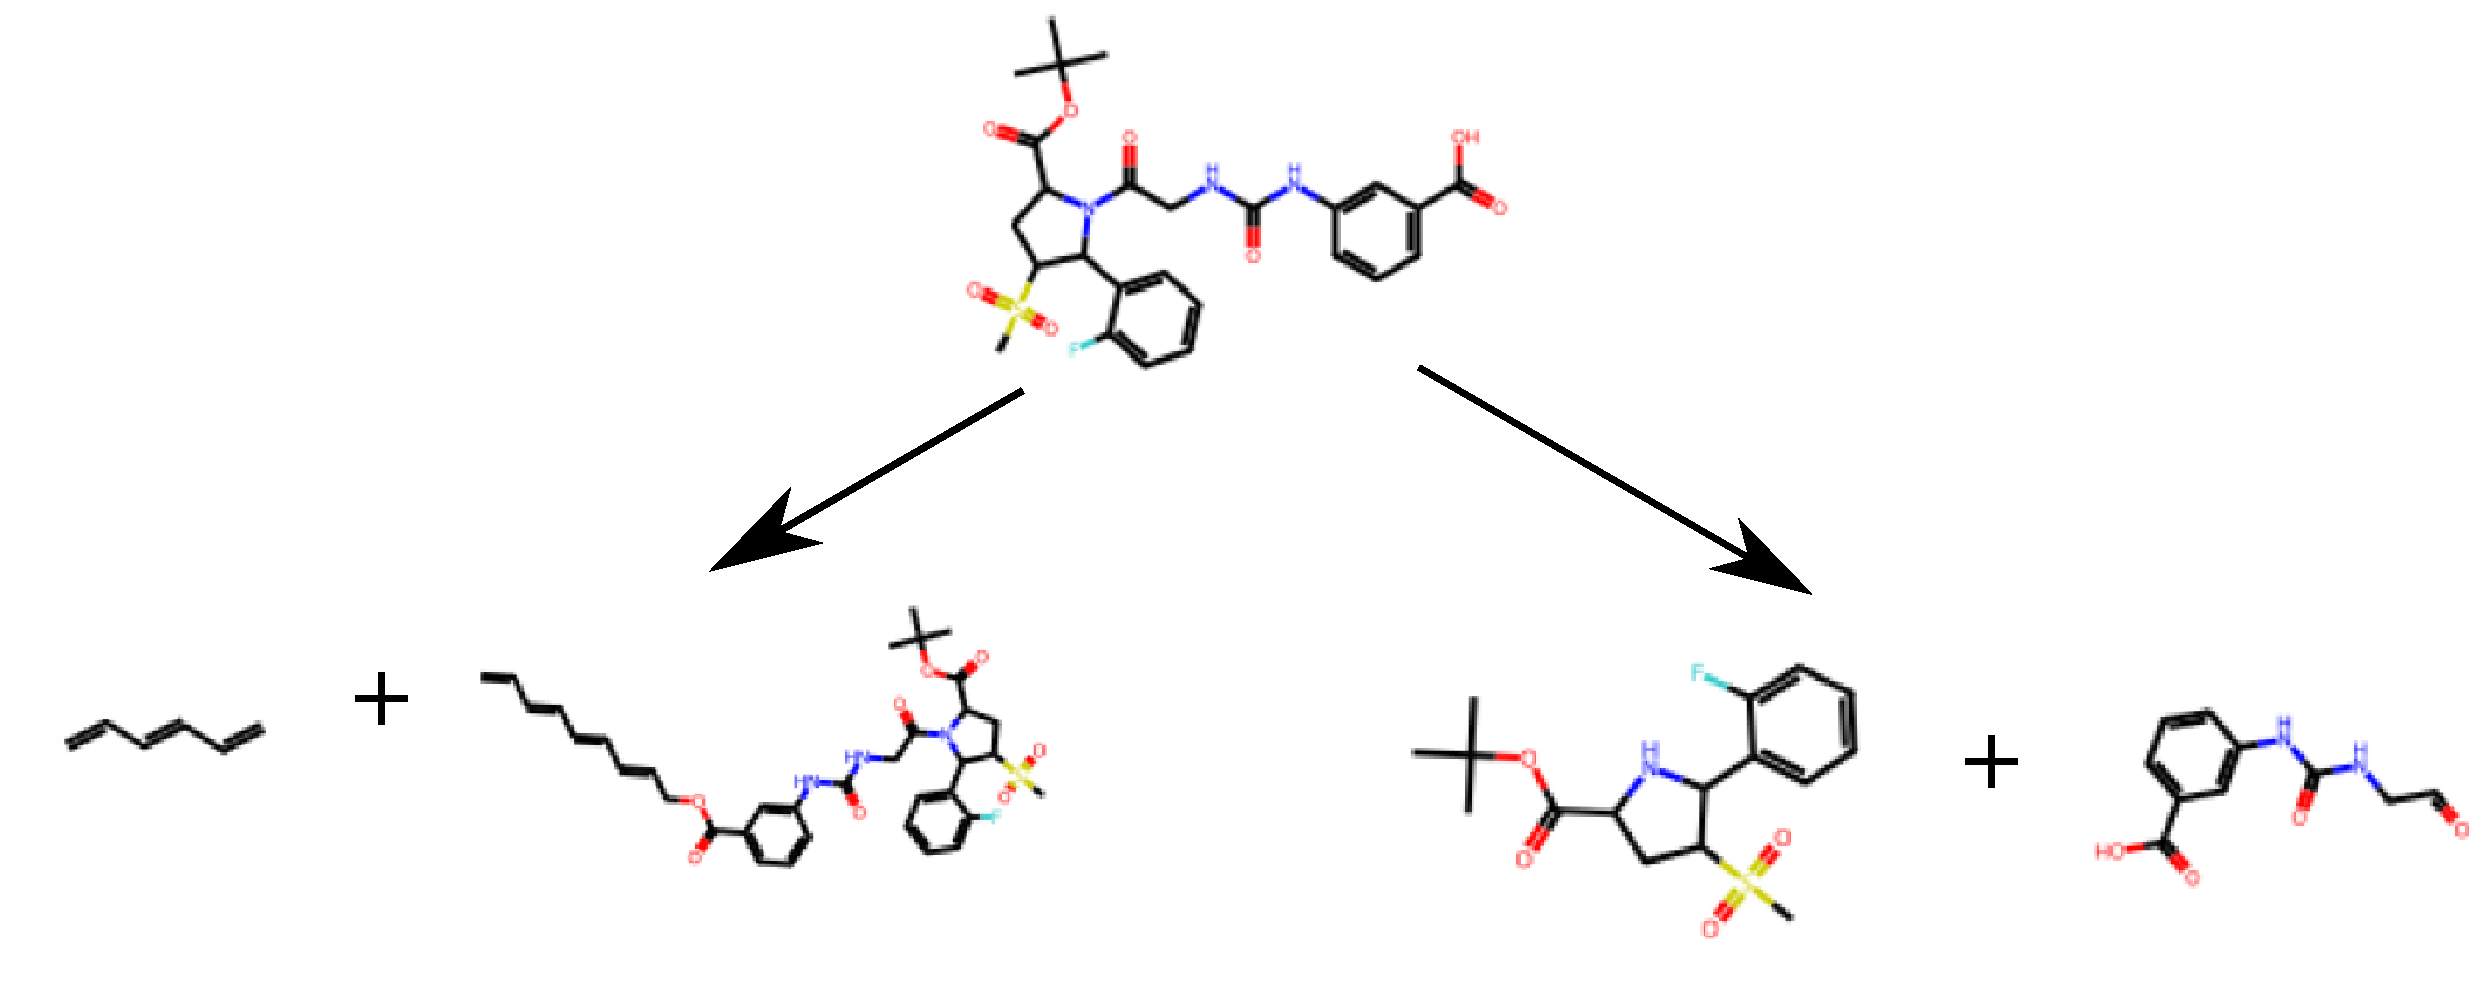
\includegraphics[width=\columnwidth]{fig/atom_guidance_small_nolabel.pdf}};

    \begin{scope}[x={(image.south east)},y={(image.north west)}]

    \node at (.5,1.02) {\textbf{Product}};
    \node at (.2,0.58) {\textbf{High atom count}};
    \node at (.2,0.5) {\textbf{guidance}};
    \node at (.8,0.58) {\textbf{Low atom count}};
    \node at (.8,0.5) {\textbf{guidance}};

    \end{scope}
    \end{tikzpicture}

\end{document}